\documentclass{ctexart}
\usepackage{acta_physica_sinica}
\usepackage{zhlipsum, lipsum}


\title[
    English Title\superscript{*}
]{
    中文标题\superscript{*}(简短明确,基金资助有上标*)
}
\author[
    David He\superscript{1)\dagger} \and Jackman He\superscript{2)} \and Cooper Guo\superscript{3)} \and John He\superscript{4)} \and Orange Guo\superscript{5)}
]{
    大维\superscript{1)\dagger} \and 杰汉\superscript{2)} \and 橙子\superscript{3)} \and 君君\superscript{4)} \and 橘子\superscript{5)}
}
\institude[
    1) Department of Micro/Nano Electronics Minhang Institute of Technology, Shanghai China

    2) School of Physics, Liberal Arts College of Zhongguan Village, Beijing China

    3) Shanghai Institute for Advanced Studies, Nanqi Technical School, Hefei China
    
    4) School of Physics, Dual-Duck Mountain University, Guangzhou China

    5) Institute of Physics, Chinese Academy of Magic, Beijing China
]{
    1)闵行理工学院 \ 微纳电子学系,上海

    2)中关村文理学院\ 物理学院,北京

    3)南七技校\ 上海研究院,上海

    4)双鸭山大学\ 物理学院,广州 

    5)中国魔法院\ 物理所,北京
}




\begin{document}
    

    \maketitle
    \abstract{
        中文摘要部分.\Blue{[300—400字,摘要中不用缩略词,不用第一人称.中英文摘要的结构建议包括:(1)研究背景和目的;(2)方法;(3)主要结果;(4)结论.简明扼要不分段,突出结论、成果]}
    }
    \keywords{宇生中微子,我家的茄子,风扇的转子,一只蛋}

    \vspace{1em}
    \pacs{42.81.Wg, 42.82.Et,01.50.Qb,01.55.+b}
    \fund{国家重点基础研究发展计划(批准号:2011CB00000)、国家自然科学基金(批准号:50875132,60573172)和国家高技术研究发展计划(批准号:2011AA06Z228)资助的课题.}

    \vspace{1em}
    \email{ddddavid@physics.org}
    \email[第一作者]{ddddavid@physics.org}

    
    \section{第一节}


    \subsection{第2部分}
    \zhlipsum[1]

    \subsubsection{第(3)点}

    \zhlipsum[3]
    一些文字 \highlight{高亮的一些文字} 还有另外一些文字

    再来一个有标题的图像占位符 图\ref{fig:标题}
    \hpic[标题]
    
    《物理学报》由中国物理学会和中国科学院物理研究所主办的综合性物理学中文学术期刊\cite{RN11},为半月刊,被SCI-CD、SCI-E、Scopus、EI、CA、INSPEC、JICST、AJ、MR等国际核心检索系统收录。 《物理学报》创刊于1933年的《中国物理学报》,1953年更名为《物理学报》

    \begin{figure}[H]
        \centering
        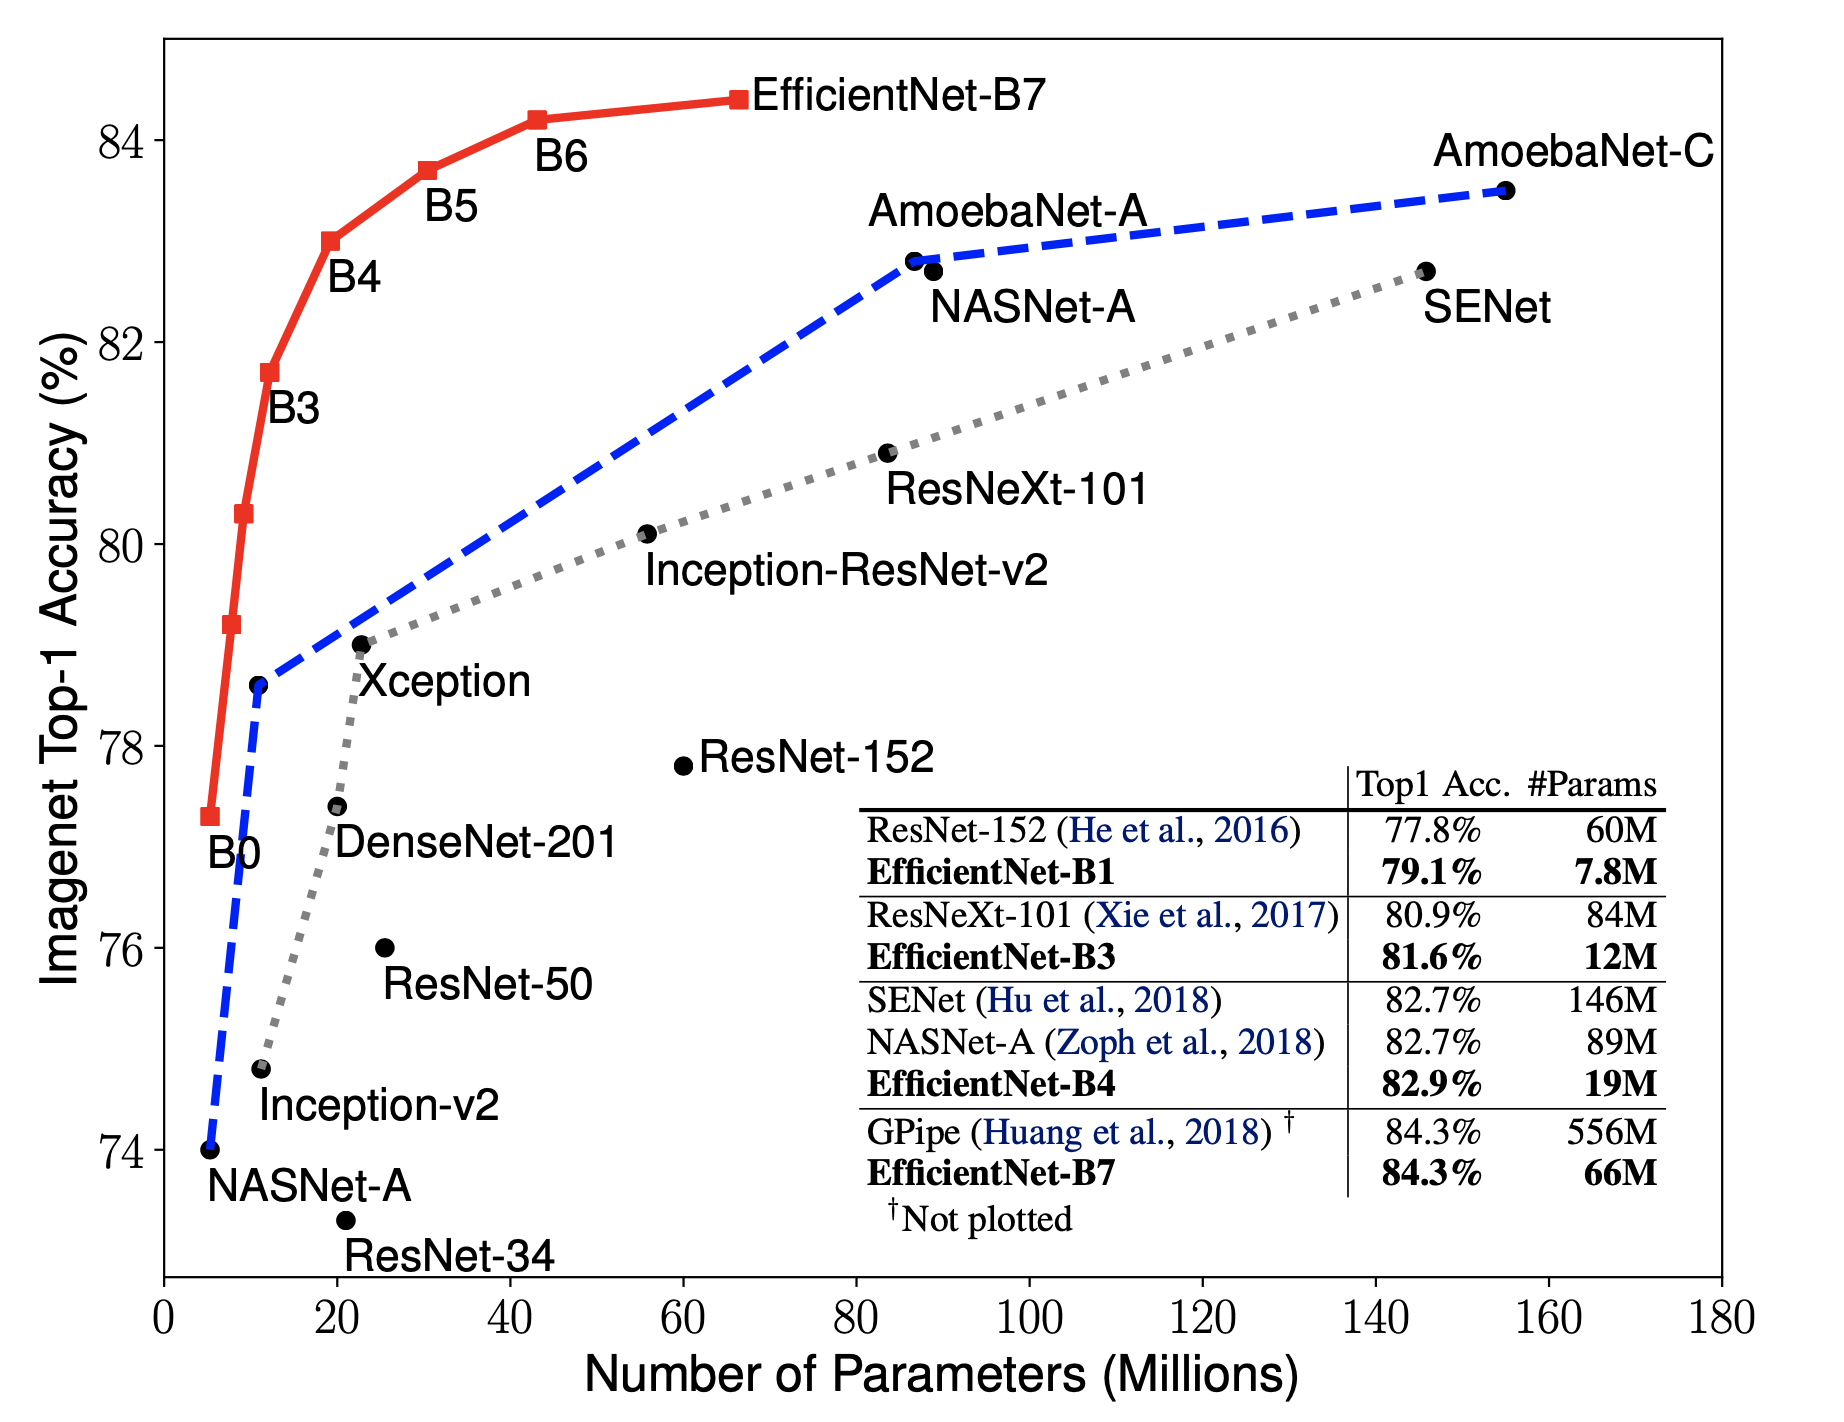
\includegraphics[width=.6\linewidth]{./figures/figure1.png}
        \bicaption{一张图}{A Figure}
    \end{figure}
    
    \begin{table}[H]
    \centering
    \begin{tabu}{.6\linewidth}{
        X[1,c] X[2,c] X[3,c] 
    }
        \toprule
        A & B & C \\
        \cline{2-3}
        1 & \SetCell[c=2]{c,m} 2\&3 \\
        \midrule
        \romannumeral1 & \romannumeral2 & \romannumeral3 \\
        piggy & eggy & honey \\
        \SetCell{bg=red, fg=white} red &
        \SetCell{bg=yellow, cmd=\fbox} yellow &
        \SetCell{bg=blue} blue \\
        \bottomrule
    \end{tabu}
    \bicaption{标题}{caption}
    \end{table}



    \section{结论}
    
    \Blue{(在研究结果与讨论的基础上总结出本研究得到的重要论点,建议可包括以下内容:(1)解释结果;(2)将结果与之前提出的研究目的或假设相联系,阐明结果的重要性;(3)将结果与其他已有研究工作进行比较;(4)尽可能得出一个很清晰的结论.对每一个结论需要总结证据。同时也可以指出本工作的不足和将要开展工作的展望。请注意不能简单重复摘要和引言.)}

    \acknowledgment{感谢北京大学尤教授和清华大学陈教授的讨论。}


    \appendix[newpage]

    \Blue{标题排列和编号方式为附录A,附录B,附录C。}

    $\pi = $ 

    3.14159 26535 89793 23846 26433
    83279 50288 41971 69399 37510
    58209 74944 59230 78164 06286
    20899 86280 34825 34211 70679
    82148 08651 32823 06647 09384
    46095 50582 23172 53594 08128
    48111 74502 84102 70193 85211
    05559 64462 29489 54930 38196
    44288 10975 66593 34461 28475
    64823 37867 83165 27120 19091
    45648 56692 34603 48610 45432
    66482 13393 60726 02491 41273

    \begin{table}[H]
        \centering
        \begin{tabu}{.6\linewidth}{
            X[1,c] X[2,c] X[3,c] 
        }
            \toprule
            A & B & C \\
            \cline{2-3}
            1 & \SetCell[c=2]{c,m} 2\&3 \\
            \midrule
            \romannumeral1 & \romannumeral2 & \romannumeral3 \\
            piggy & eggy & honey \\
            red & yellow & blue \\
            \bottomrule
        \end{tabu}
        \caption{第零个表格}
    \end{table}


    \appendix

    \Blue{每个附录里如果有表,则相应为表A1,A2,表B1,B2,表C1,C2。}

    \begin{table}[H]
        \centering
        \begin{tabu}{.6\linewidth}{
            X[1,c] X[2,c] X[3,c] 
        }
            \toprule
            A & B & C \\
            \cline{2-3}
            1 & \SetCell[c=2]{c,m} 2\&3 \\
            \midrule
            \romannumeral1 & \romannumeral2 & \romannumeral3 \\
            piggy & eggy & honey \\
            red & yellow & blue \\
            \bottomrule
        \end{tabu}
        \caption{第一个表格}
    \end{table}

    \begin{table}[H]
        \centering
        \begin{tabu}{.6\linewidth}{
            X[1,c] X[2,c] X[3,c] 
        }
            \toprule
            A & B & C \\
            \cline{2-3}
            1 & \SetCell[c=2]{c,m} 2\&3 \\
            \midrule
            \romannumeral1 & \romannumeral2 & \romannumeral3 \\
            piggy & eggy & honey \\
             red & yellow & blue \\
            \bottomrule
        \end{tabu}
        \bicaption{双语也行}{Dual Language Title}
    \end{table}



\newpage

    \maketitle
    \abstract[english]{
        To determine the probe made of amino acids arranged in a linear chain and joined together by peptide bonds between the carboxyl and amino groups of adjacent amino acid residues. The sequence of amino acids in a protein is defined by a gene and encoded in the genetic code. This can happen either before the protein is used in the cell, or as part of control mechanisms. 
    }
    \keywords[english]{
        neutrino, spinner, eggplant, egg
    }
    \fund[english=true]{Project supported by the State Key Development Program for Basic Research of China (Grant No. 2011CB00000), the National Natural Science Foundation of China (Grant Nos. 50875132,60573172 ), and the National High Technology Research and Development Program of China ( Grant No.2011AA06Z228 ) .}


    
    \bibreference[
        nocite, % 如果需要展示所有(包括未引用)的条目,加上这个参数
        newpage
    ]{bibfile}

    

\end{document}

